\documentclass{article}

\usepackage[utf8]{inputenc} % allow utf-8 input
\usepackage[T1]{fontenc}    % use 8-bit T1 fonts
\usepackage{hyperref}       % hyperlinks
\usepackage{url}            % simple URL typesetting
\usepackage{booktabs}       % professional-quality tables
\usepackage{amsfonts}       % blackboard math symbols
\usepackage{nicefrac}       % compact symbols for 1/2, etc.
\usepackage{microtype}      % microtypography

\usepackage{graphicx}
\usepackage{subcaption}
% \captionsetup{skip=0.25\baselineskip}
% \captionsetup[subfigure]{skip=1pt, singlelinecheck=false}
\usepackage[leftcaption]{sidecap}

% \setlength{\parindent}{0pt}

\usepackage{geometry}
\geometry{margin=1in}

\usepackage{float}
\usepackage{csc}
\newtheorem{definition}{Definition}
\usepackage{enumitem}

\title{CSC2412 Project: DPGAN and Model Inversion}
\author{Jason Tang}
\date{April 15, 2023}

\usepackage[skip=10pt plus1pt, indent=20pt]{parskip}

\begin{document}
\maketitle

% Abstract
\begin{abstract}
    The growing concern over privacy in data-driven applications has led to the development of various privacy-preserving techniques, including Differential Privacy for Model Inversion (DPMI) \cite{dpmi}. DPMI has shown promise in generating synthetic data for privacy-preserving applications using Generative Adversarial Networks (GANs), which often suffer from issues such as mode collapse and long training times. In this project, we explored the use of autoencoders and Variational Autoencoders (VAEs) as potential alternatives to GANs in the DPMI framework. We conducted experiments to compare the performance of autoencoders and VAEs with GANs in terms of stability, privacy, and utility, using evaluation metrics such as Inception Score (IS) and Fréchet Inception Distance (FID). Overall, our findings suggest that autoencoders and VAEs offer simplicity and stability compared to GANs, and show potential as viable GAN alternatives in situations when GANs are too unstable or expensive to train.
\end{abstract}

\section{Introduction}

\parindent=20pt With advances in information technology and mobile computing, increasing amounts of consumer data are being collected and utilized to train machine learning models. Though the widespread utility of these models is undeniable, both ethical and legal concerns arise due to the combination of sensitive portions of the data, and the susceptibility of large machine learning models to membership attacks \cite{mi_attack}. Differential privacy (DP) presents a solution to these data sensitivity issues in the form of formal privacy guarantees, and is commonly applied by adding gaussian noise during the training process, such as in DP-SGD \cite{dpsgd}. 

These methods have become increasingly popular for privately training and releasing models for downstream tasks, but lack the ability to release any datasets, as the original private data remains unaltered. One alternative is to release a synthetic dataset or generative model under differential privacy to train non-private downstream models, as the privacy of the original sensitive data is protected through DP post-processing. This dataset releasing method is simple to integrate into standard non-private training pipelines as a data input modification, can be combined with other datasets to train stronger models, and allows the safe transfer of sanitized data to other researchers for the development of new technologies.

Within deep learning, generative models such as autoencoders and generative adversarial networks (GANs) are often released to generate synthetic data for downstream applications. In this project, we will explore several proposed differentially private generative models and to evaluate the empirical effects of potential improvements.



\section{Related Work}
\newcommand{\M}{\mathcal{M}}
\newcommand{\D}{\mathcal{D}}
\newcommand{\RR}{\mathcal{R}}

% %%%%%%%%%%%%%%%%%%%%%%%%%%%%%%%%%%%%%%%%%%%%%%%%%%%%%%%%%%%%%%%%
\subsection{DP-SGD}
Differential privacy (DP) presents a solution to these data sensitivity issues in the form of formal privacy guarantees, and is commonly applied by adding gaussian noise during the training process, such as in DP-SGD \cite{dpsgd}. In this seminal paper, Abadi et al. present a differentially private method for training deep neural networks by adding random noise to clipped gradient updates, both of which are necessary for provable privacy guarantees. Since the noise is gaussian, this leads to $(\epsilon, \delta)$-DP, which is defined as follows:
\begin{definition}
	A randomized mechanism $\M : \D \rightarrow \R$ with domain $\D$ and range $\RR$ satisfies $(\epsilon, \delta)$-differential privacy if for any two adjacent inputs $d, d' \in \D$ and for any subset $S \subset \RR$ it holds that
\[
	\pr{\M(d) \in S} \leq e^\epsilon \pr{\M(d') \in S} + \delta
\]
\end{definition}
Additionally, we define sampling probability $q = L/N$, where $L$ is the batch size of examples averaged before adding noise, and $N$ is the total number of examples.

They also introduce the moment account method, which provides a tighter worst case privacy bound compared to strong composition, allowing for lower privacy costs during each iteration. Specifically, they reduce the strong composition privacy bound $(\cO(q\epsilon\sqrt{T\log(1/\delta)}), Tq\delta)$ to the moments accountant bound $(\cO(q\epsilon\sqrt{T}), \delta)$. Which is significant as $\delta$ is usually very small, and $T \gg 1/q$ as each training example is used multiple times. The resulting $(\epsilon, \delta)$ differential privacy is useful as it provides graceful degradation, robustness to auxiliary information, and can easily be combined with other methods due to the composition theorem.


% %%%%%%%%%%%%%%%%%%%%%%%%%%%%%%%%%%%%%%%%%%%%%%%%%%%%%%%%%%%%%%%%
\subsection{Tempered Sigmoids}
One issue with using DP-SGD to train deep learning models is the commonly used ReLU activation function and its unbounded range. Papernot et al. \cite{sig} observe that the lack of a bound on model activations leads to exploding gradients, which, when combined with the gradient clipping of DP-SGD, leads to low utility gradient updates. As such, the authors propose using a family of bounded functions called tempered sigmoids instead of ReLUs as activation functions to enhance performance. They demonstrate that the use of tempered sigmoids allows for explicit control of the gradient norm and model sensitivity. This is evidenced by empirical results which demonstrate faster convergence and the reduction of negative impacts caused by clipping and adding noise to large gradients.


% %%%%%%%%%%%%%%%%%%%%%%%%%%%%%%%%%%%%%%%%%%%%%%%%%%%%%%%%%%%%%%%%
\subsection{Feature Extraction}
Tramèr and Boneh \cite{features} demonstrate an effective baseline method based on extracting non-learned handcrafted features from private images using Scatternet \cite{scatter} (a SIFT-like feature extractor). Due to the reduction in dimensionality, this method requires far fewer iterations to converge, and as such, allows practitioners to inject less noise into each gradient step for the same differential privacy guarantees. As a result of this baseline, the authors suggest that differentially private learning can achieve model performance comparable to non-private learning by exploring two potential directions: designing non-learned features or pretraining on public data.

As such, most of the recent methods developed for private image classification focus on utilizing pretrained weights learned on public data and fine tuning only the last layers in a private manner \cite{transfer} \cite{2nd_order}. One such method is presented by Mehta et al. \cite{2nd_order}, which explores more sophisticated second-order optimization methods such as Newton’s method to privately tune the last layer of a pretrained model learned on public data. In particular, they introduce a training method known as DP-FC, which utilizes feature covariance instead of the hessian as second order information, and performs especially well with smaller epsilon values (< 1). Another recent method by Mehta et al. is “Large Scale Transfer Learning for Differentially” \cite{transfer}, which explores using the LAMB optimizer for last layer fine tuning, which is intended to perform well with large batch sizes, and analyzes single step training in the full batch setting.




\newcommand{\ww}{\textbf{w}}
\newcommand{\xx}{\textbf{x}}
\newcommand{\xxh}{\hat{\textbf{x}}}
\newcommand{\zz}{\textbf{z}}

% %%%%%%%%%%%%%%%%%%%%%%%%%%%%%%%%%%%%%%%%%%%%%%%%%%%%%%%%%%%%%%%%
\subsection{DPGAN}

The popularity of GANs has surged in recent times due to their remarkable capacity to hallucinate lifelike images. However, the highly expressive nature of non-private GANs makes them susceptible to memorizing the training data. To address this, Xie et al. propose a differentially private generative adversarial network (DPGAN) \cite{dpgan} that protects the privacy of training data using a WGAN architecture \cite{wgan}, which solves the following minimax game:
\[
    \min_{G} \max_{\ww \in W} \EE_{\xx \sim p_{data}(\xx)} [f_\ww (\xx)] - \EE_{\zz \sim p_{\zz} (\zz)} [f_\ww (G(\zz))]
    \tag{1}
\]
where $G$ is the generator, $f_\ww$ is the discriminator ($\ww$ are its parameters), $p_{data}(\xx)$ is the real data distribution, $p_{\zz} (\zz)$ is a gaussian distribution, and $W$ is the set of all possible parameters for $\ww$. 
This results in the following losses which are minimized:
\begin{align*}
    \mathcal{L}_D &= -\EE_{\xx \sim p_{data}(\xx)} [f_\ww (\xx)] + \EE_{\zz \sim p_{\zz} (\zz)} [f_\ww (G(\zz))]
    \tag{2}
    \\
    \mathcal{L}_G &= -\EE_{\zz \sim p_{\zz} (\zz)} [f_\ww (G(\zz))] 
    \tag{3}
\end{align*}
Additionally, WGAN sets the constraint that all $f_\ww(x)$ are $K$-Lipschitz (with respect to $x$) for some $K$, i.e. their weights are clipped.

As a result of this weight clipping, the authors are able to replace the DP-SGD gradient clipping with explicitly defined gradient bounds from weight clipping (Lemma 3.5 in the paper):
\[
    \norm{g_\ww (\xx^{(i)}, \zz^{(i)})} \leq 2 c_p B_\sigma B_{\sigma'}^2 \sum_{k=1}^{H-1} m_k m_{k+1} 
    \tag{4}
\]
where $g_\ww$ is the gradient of the discriminator's parameters $\ww$ with respect to the Wasserstein loss, $c_p$ is the weight clipping constant, $B_\sigma$ is the range bound on activation functions ($\sigma(\cdot) \leq B_\sigma$), $B_{\sigma'}$ is the bound on activation derivatives ($\sigma'(\cdot) \leq B_{\sigma'}$), $m_k$ is the number of neurons in layer $k$, and $H$ is the number of non-input layers in the discriminator (assuming a fully connected network).

Their proposed algorithm guarantees $(\epsilon, \delta)$ differential privacy using the Moments Accountant from DP-SGD \cite{dpsgd} and is shown to be effective in generating reasonable MNIST images, albeit at relatively high $\epsilon$’s (in the range [9.6, 29.0]).
Additionally, the use of WGAN over a traditional GAN \cite{gan} using Jensen-Shannon divergence helps stabilize training and generally avoids issues such as mode collapse.



% %%%%%%%%%%%%%%%%%%%%%%%%%%%%%%%%%%%%%%%%%%%%%%%%%%%%%%%%%%%%%%%%
\subsection{DP Model Inversion}

Despite the stability improvements, learning a GAN from scratch is still a lengthy process which requires hundreds of thousands of iterations to converge, which requires large amounts of noise to gradients to maintain the same privacy guarantees. One way to improve the training efficiency of complex DP-GANs is through dimensionality reduction \cite{stable_gan}. Chen et al. explore this idea in “Differentially Private Generative Adversarial Networks with Model Inversion” (DPMI) by first publicly training an Improved-WGAN \cite{improved_wgan}, which uses gradient norm penalty instead of weight clipping. This is done by changing the losses to:
\begin{align*}
    \mathcal{L}_D &= -\EE_{\xx \sim p_{data}(\xx)} [f_\ww (\xx)] + \EE_{\zz \sim p_{\zz} (\zz)} [f_\ww (G(\zz))] + \lambda \left( \norm{ \nabla_{\xxh} f_{\ww}(\xxh) }_2 - 1\right)^2
    \tag{5}
    \\
    \mathcal{L}_G &= -\EE_{\zz \sim p_{\zz} (\zz)} [f_\ww (G(\zz))]
    \tag{6}
\end{align*}
where $\xxh = c \xx + (1-c) G(\zz)$, $c \sim U[0, 1]$ is random number, and $\lambda$ is the gradient penalty coefficient. This imposes a soft constraint towards 1-Lipschitz on the discriminator.

The authors then perform model inversion using gradient ascent on the resulting public generator to compute the closest latent space representation of the private data points \cite{dpmi}. To do so, they follow this optimization process (Equation (4) in the paper): 
\begin{align*}
    z_s &= \text{argmin}_{z} \norm{G(z) - \xx}^2
    \tag{7}\\
    &\text{s.t. } P_Z (z) \geq P_Z (z_0)
\end{align*}
where $z_0 \sim P_Z = \mathcal{N}^d(0, I)$, where $d$ is the size of the latent dimension. This convex constraint ensures that the latent vector $z_s$ is of a quality comparable to $G(z_0)$. The solution to this optimization problem is found through projected gradient ascent.

These private latent vectors are then used to learn a standard DP-GAN in the lower-dimensional latent space, leading to fewer iterations necessary for convergence and less additive noise for the same privacy guarantees. The final DP-GAN generator can then be released to generate synthetic latent vectors, which can then be inputted into the original public GAN to generate synthetic images approximating to those within the private dataset.

The authors also compare the standard DP-SGD paradigm to Private Aggregation of Teacher Ensembles (PATE) \cite{pate}, which uses multiple models trained on disjoint subsets of sensitive data as teachers for a student model. The student model learns to predict an output chosen by noisy voting among all of the teachers, and cannot directly access an individual teacher or the underlying data or parameters. The student model then learns to predict outputs chosen through noisy voting among multiple teachers, without having direct access to teacher models or underlying data. As a result, this method is able to impose only weak assumptions on the teacher model architectures or training processes, which provides much more flexibility compared to DP-SGD based methods. However, PATE-based training methods tend to be data inefficient because they require training multiple teacher models on separate sets of data, which can be challenging with small datasets commonly encountered in real-world scenarios. As a result, the authors of DPMI chose to adopt DP-SGD despite the limitations imposed on the potential models.



\subsection{DP Autoencoders}
In contrast to other studies that primarily focus on GAN variants, Chen et al. \cite{dp_gen} investigate the robustness of differentially private autoencoders and variational autoencoders \cite{vae} against model inversion and GAN-based adversarial attacks. They propose two models: an autoencoder-based generative model (AuGM), and a variational autoencoder generative model (VaeGM). To generate labeled synthetic data in VaeGM, the authors adopt a strategy of privately training separate variational autoencoders (VAEs) for each class using DP-SGD \cite{dpsgd}. The use of VAEs allows for infinite data generation by simply sampling random Gaussian noise, but empirical results show that it is unstable when trying to generate high-quality samples. AuGM works by first privately training an autoencoder using DP-SGD and then using the encoder of the autoencoder to synthesize information from the private data into the generated outputs. This provides stronger protection against model inversion and GAN-based attacks compared to VaeGM, but requires downstream users to have access to a large amount of related public data to pass through the encoder to generate the synthetic data.



\section{Methodology}

\begin{figure*}[!h]
    \centering
    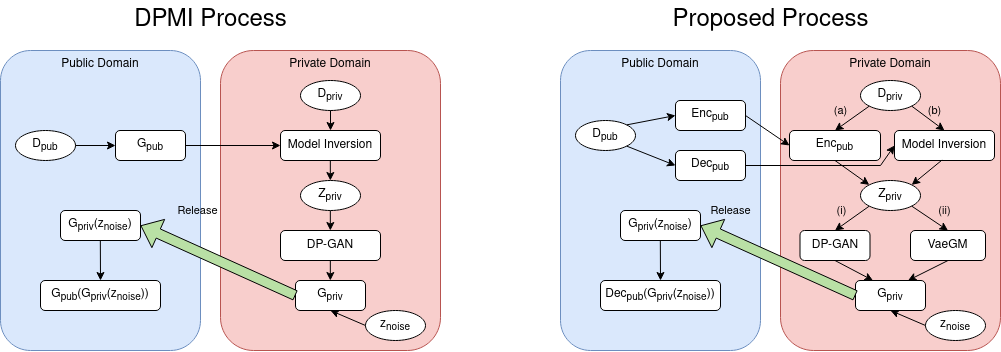
\includegraphics[width=\columnwidth]{images/setup.png}
    \caption{Diagram of the DPMI framework and our proposed modifications.}
    \label{fig:setup}
\end{figure*}

In this project, we will explore several proposed variations to the DPMI framework and empirically assess their performance (See Fig. \ref{fig:setup} for the setup). The main difference is the use of a publicly trained autoencoder (AE) instead of a GAN, which is intended to alleviate some of the issues found in GAN training, as well as provide the ability to simply encode the private data with the public encoder to get the latent representations, or use the DPMI method of gradient ascent using the public decoder (Fig. \ref{fig:setup} (a) and (b), respectively). Additionally, besides the DP-GAN \cite{dpgan} used to generate synthetic latent vectors, we also consider a single-class version of VaeGM \cite{dp_gen} since we don’t require labels (Fig. \ref{fig:setup} (i) and (ii), respectively). 

% Create table summarizing the naming conventions
\begin{table}
    \centering
    \begin{tabular}[!h]{|c|c|c|c|}
        \hline
        \textbf{Public Method} & \textbf{Latent Extraction Method} & \textbf{Private Learning Method} & \textbf{Abbreviation}\\
        \hline
        GAN & Gradient Ascent & DP-GAN & wgan-GAN (DPMI)\\
        \hline
        GAN & Gradient Ascent & VaeGM & wgan-VAE\\
        \hline
        Autoencoder & Encoder & DP-GAN & ae-enc-GAN\\
        \hline
        Autoencoder & Encoder & VaeGM & ae-enc-VAE\\
        \hline
        Autoencoder & Gradient Ascent & DP-GAN & ae-grad-GAN\\
        \hline
        Autoencoder & Gradient Ascent & VaeGM & ae-grad-VAE\\
        \hline
    \end{tabular}
    \caption{Naming conventions for the different methods.}
    \label{fig:naming}
\end{table}

Overall, the aim of this project is to explore substituting GANs with simpler, more stable models such as autoencoders and VAEs which are less expressive, but avoid training issues such as mode collapse and long learning times required to generate higher quality results. Autoencoders and VAEs were chosen as they have been shown to have success in DP applications \cite{dp_gen} before, and VAEs are similar to GANs in their ability to generate an infinite amount of synthetic data once trained. Through this, we hope to provide an easier to train and more stable alternative to the DPMI framework, which can be used to generate synthetic data for applications where training GANs would be unstable.



\section{Experiments}
In our implementation, we mainly utilize PyTorch \footnote{https://pytorch.org/} for model training and data management, and Opacus \footnote{https://opacus.ai/} \cite{opacus} for privacy accounting. Our implementation is available on GitHub: \url{https://github.com/JasonTang99/csc2412_project}, and our experiment results are available on \href{https://drive.google.com/file/d/1nR0wDjarNUtH99o7XbLVs1exvMhBTxh9/view?usp=share_link}{Google Drive}.

\begin{figure*}[!h]
    \centering
    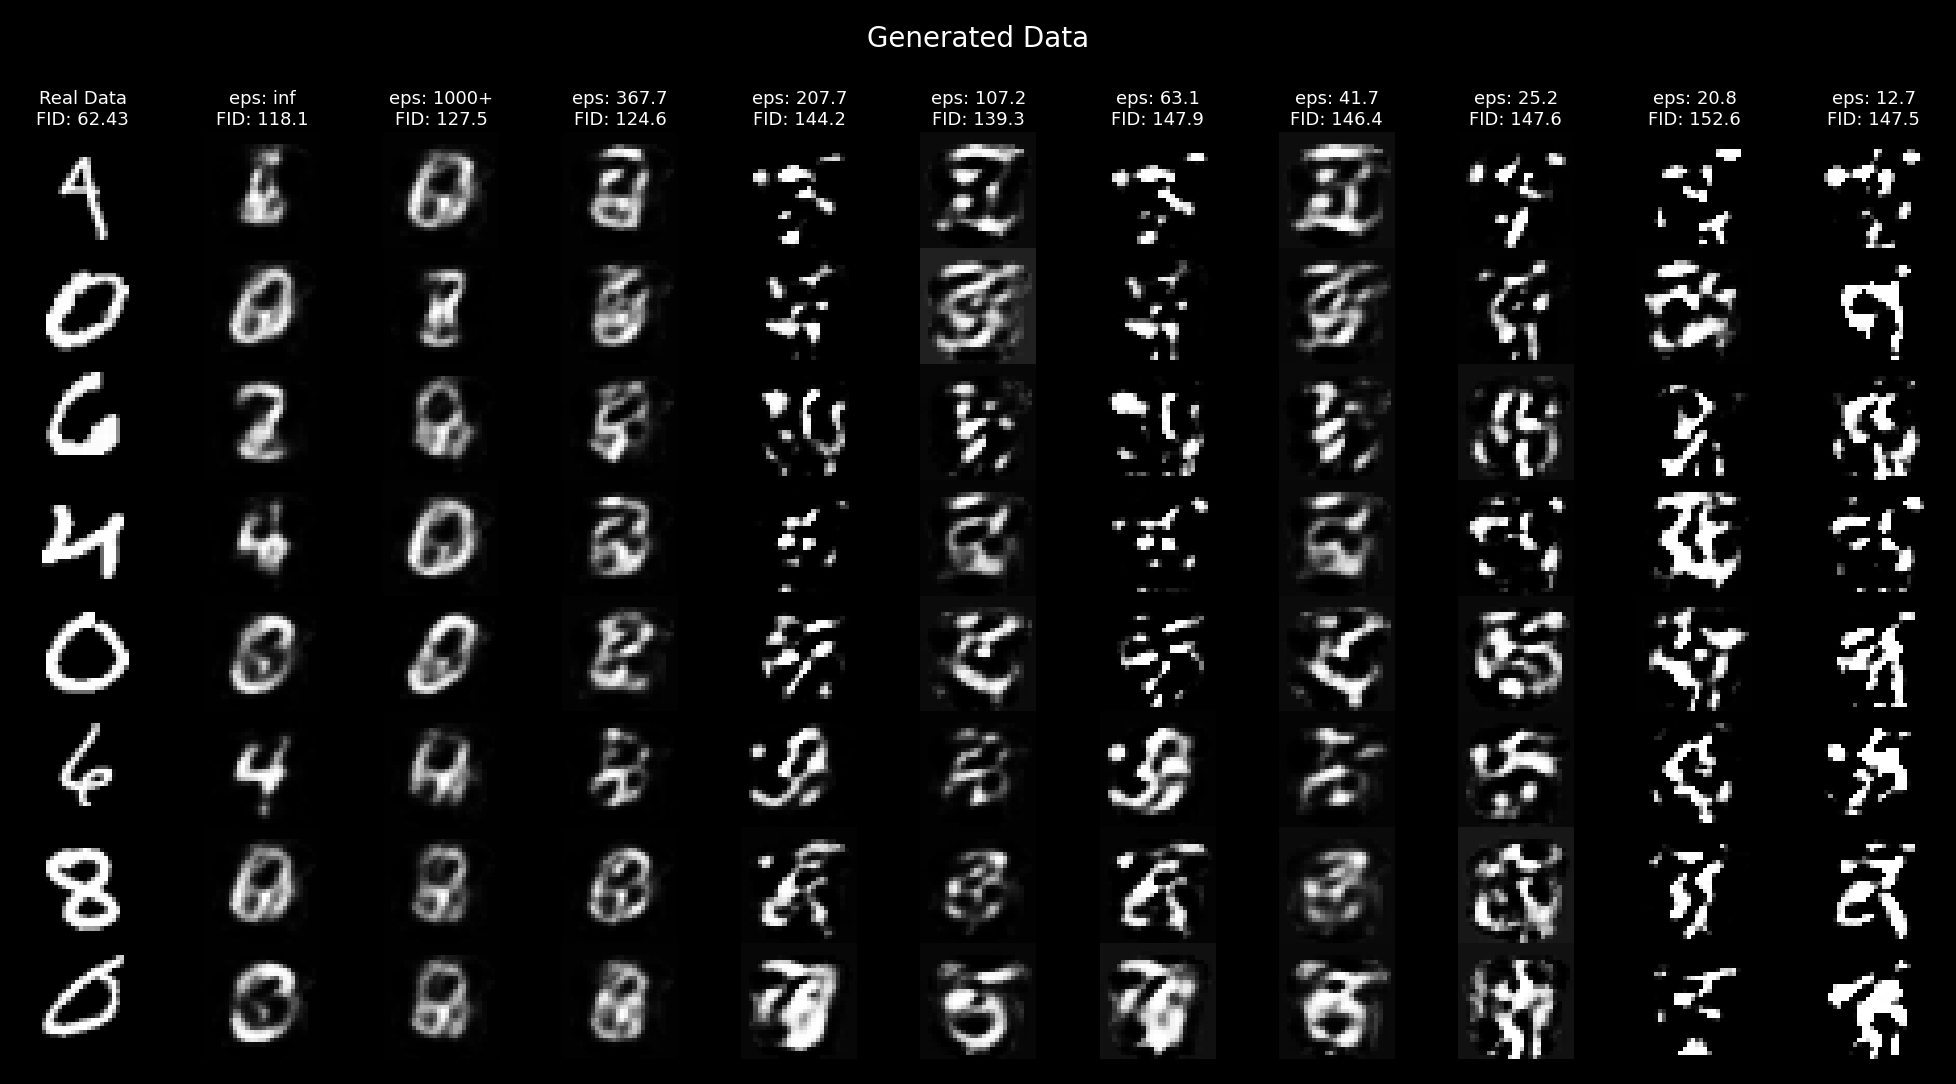
\includegraphics[width=\columnwidth]{images/generated_data.png}
    \caption{Generated data at different values of $\epsilon$ using the ae-grad-VAE model.}
    \label{fig:generated_data}
\end{figure*}
\subsection{Dataset}
We run all experiments on the MNIST dataset, which consists of 60,000 28x28 pixel grayscale images of handwritten digits. For data partitioning, we follow the method used in DPMI \cite{dpmi}:
\begin{itemize}[noitemsep]
    \item Labeling dataset: 1/3 of training data (20,000 images)
    \item Public dataset: 1/2 of classes (odd digits) in the remaining data (20,388 images)
    \item Private dataset: 1/2 of classes (even digits) in the remaining data (19,612 images)
    \item Test dataset: original test data (10,000 images)
\end{itemize}
We maintain the same random partition throughout all experiments. 

\subsection{Metrics}
We utilize the common metrics of Inception Score (IS) \cite{IS} and Fréchet Inception Distance (FID) \cite{FID} to empirically evaluate the quality of the generated data. Inception Score (IS)\cite{IS} is a metric that measures the quality and diversity of synthetic images which utilizes features extracted from a pre-trained Inception V3 network (larger is better). Frechet Inception Distance (FID) \cite{FID} is an improvement upon IS which that measures the distance between the distributions of real and synthetic images (smaller is better).

We refer to an implementation of Inception Score \footnote{https://github.com/sbarratt/inception-score-pytorch} and Fréchet Inception Distance \footnote{https://github.com/mseitzer/pytorch-fid} for our experiments.





\subsection{Hyperparameters}
We explore a range of hyperparameter settings detailed for all steps in the appendix (Table \ref{table:hyperparameters}). Due to limited time and computational resources, we were unable to explore a wider set of hyperparameters for performances comparable to the original DPMI framework. However, we believe that our results are still useful in demonstrating the stability improvements of our proposed modifications to the DPMI framework.

\begin{figure*}[!h]
    \centering
    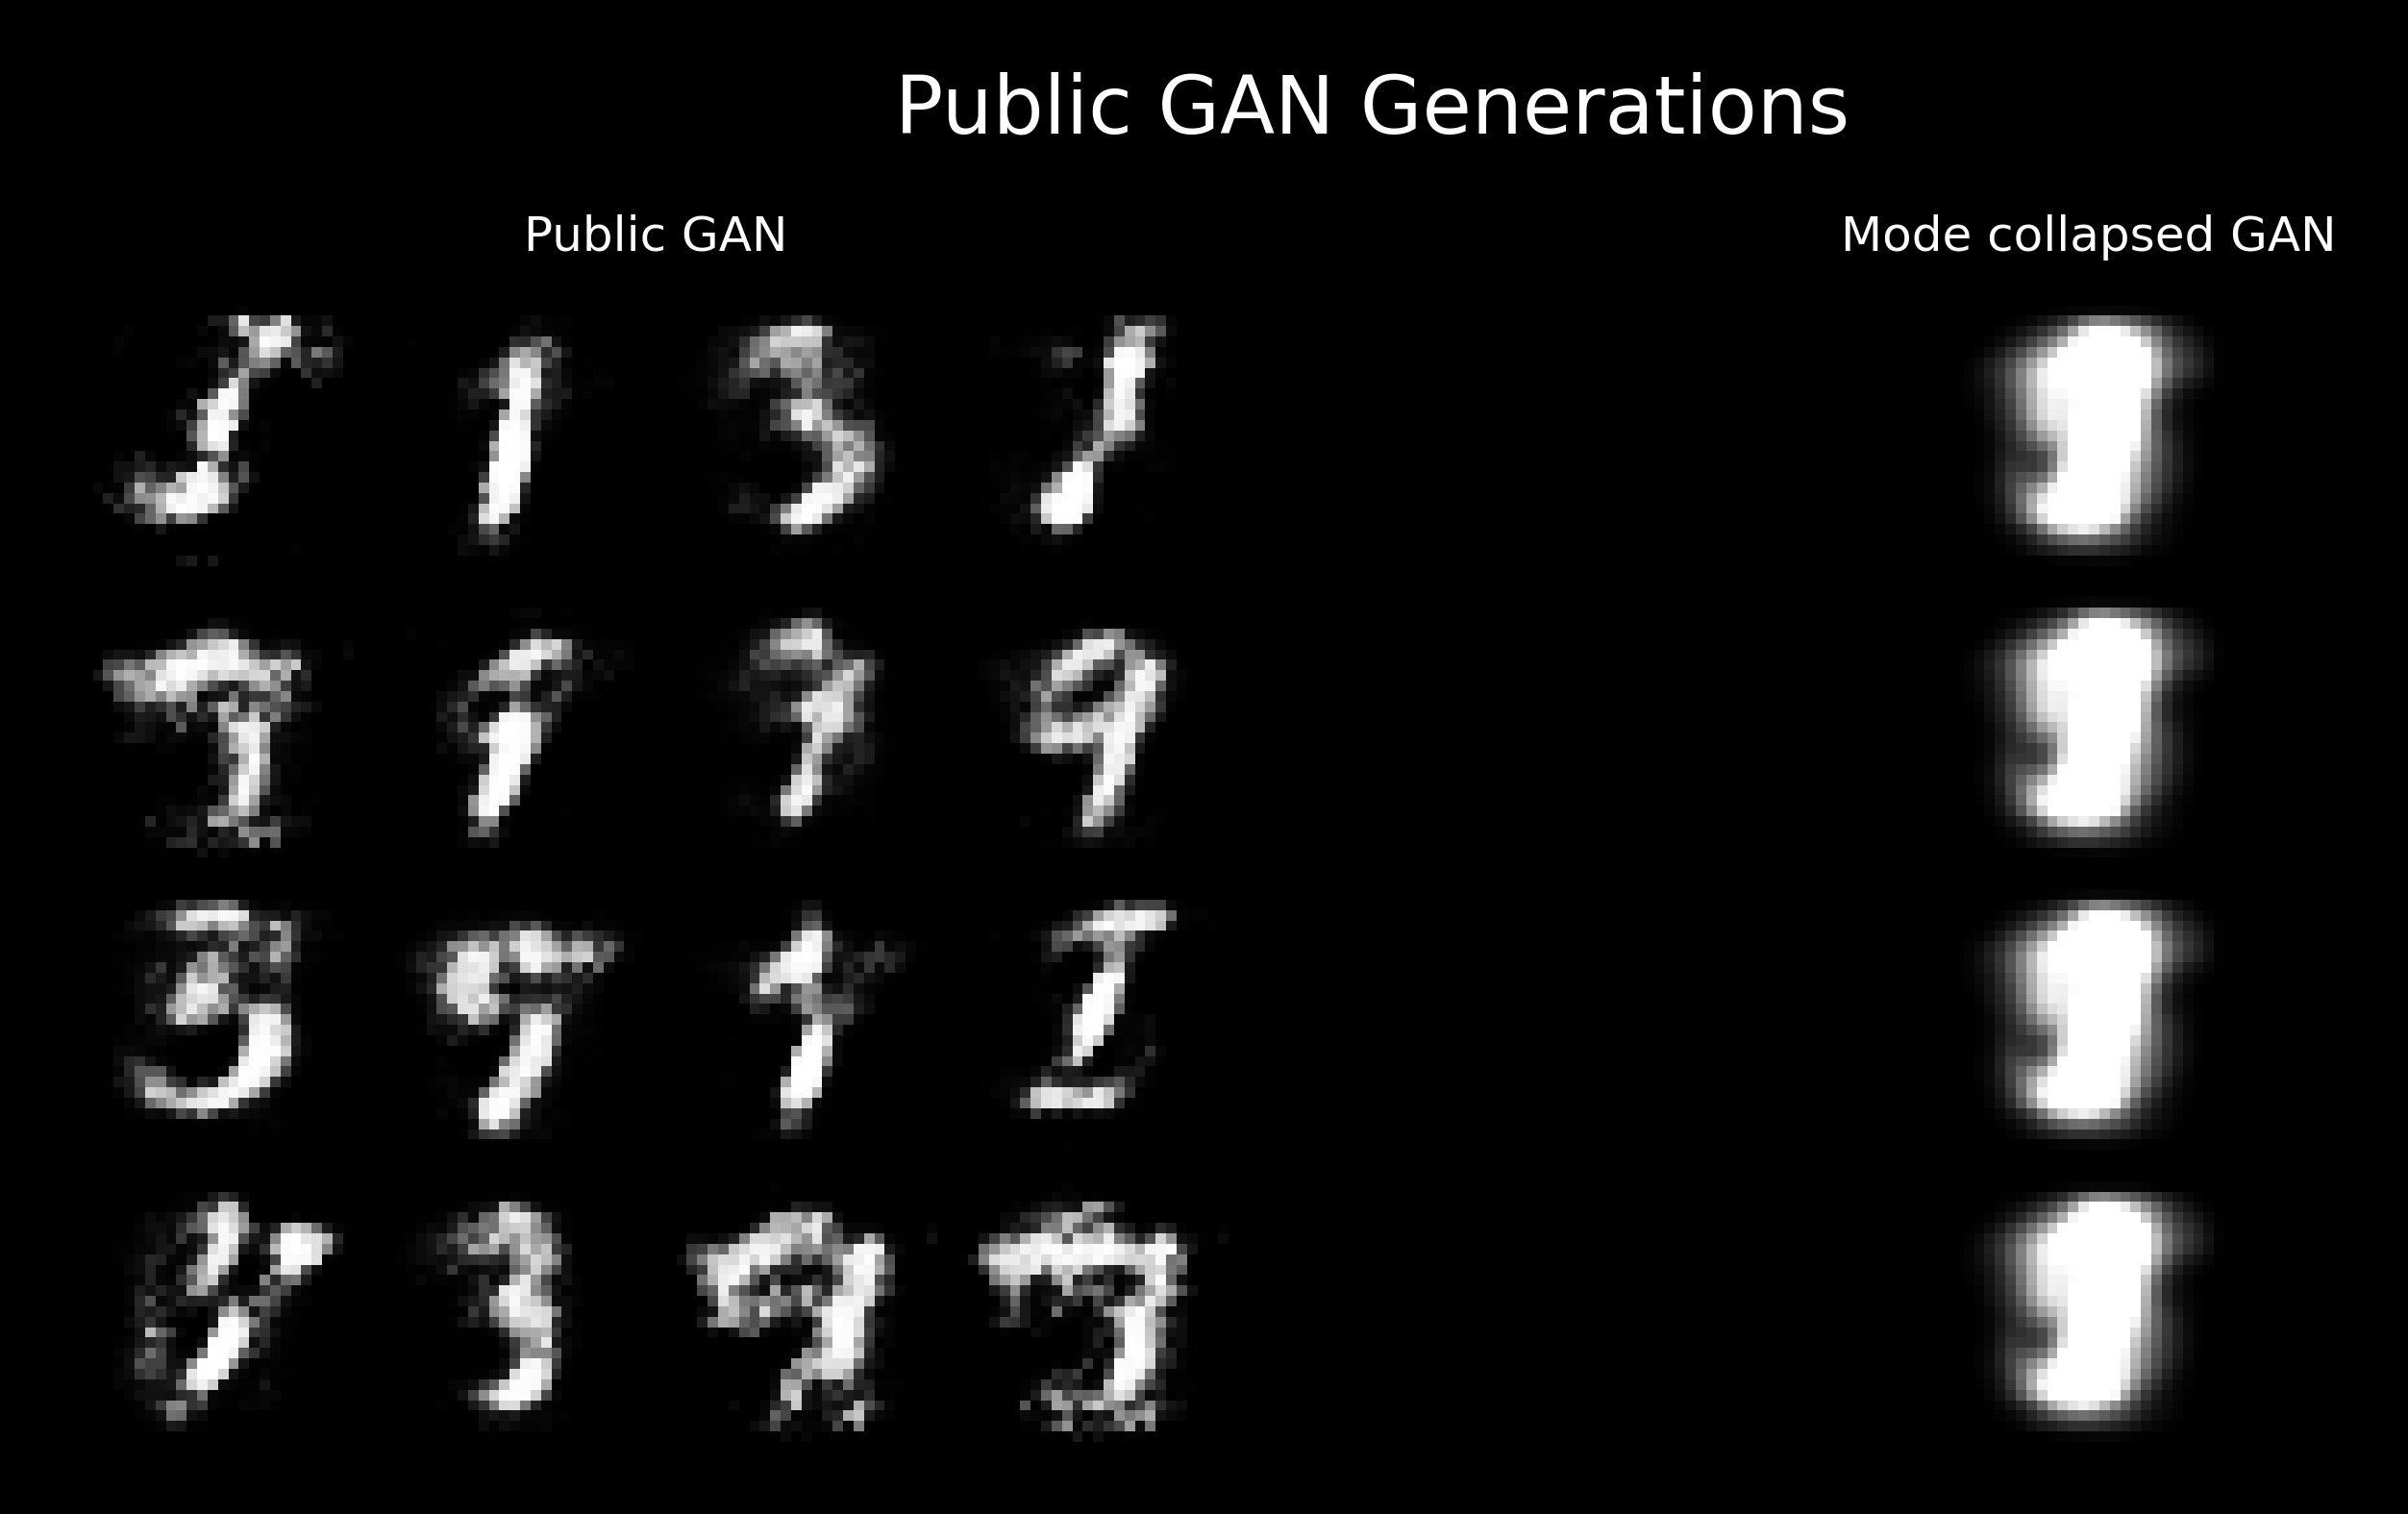
\includegraphics[width=0.7\columnwidth]{images/public_gan_training.png}
    \caption{Samples generated by the public GAN.}
    \label{fig:public_gan_training}
\end{figure*}

\subsection{GAN vs. AE Training}
Throughout our hyperparameter searches and experiments, we found it difficult to get publicly trained GANs to converge, but those that did were able to generate reasonable results for the simple fully-connected generator models we used (Fig. \ref{fig:public_gan_training}). We found that most of our attempt to publicly train GANs failed, and all of our experiments with DP-GAN (DPMI, ae-enc-GAN, ae-grad-GAN) failed to converge (Fig. \ref{fig:mode_collapse}). This could be potentially due to bugs in our code but we believe it is likely a result of insufficient hyperparameter search combined with the instability of GAN training. Moreover, each GAN training experiment would take between 2-3 hours to complete, which made it difficult to run a large number of experiments. 

Comparatively, we were able to train each version of the public autoencoder in a single experiment in under 1 hour, and each experiment with the private VaeGM took less than 10 minutes. This is likely due to the fact that autoencoders and VAEs are much simpler models than GANs, and are far more stable to train at higher learning rates. 


\begin{figure*}[!h]
    \centering
    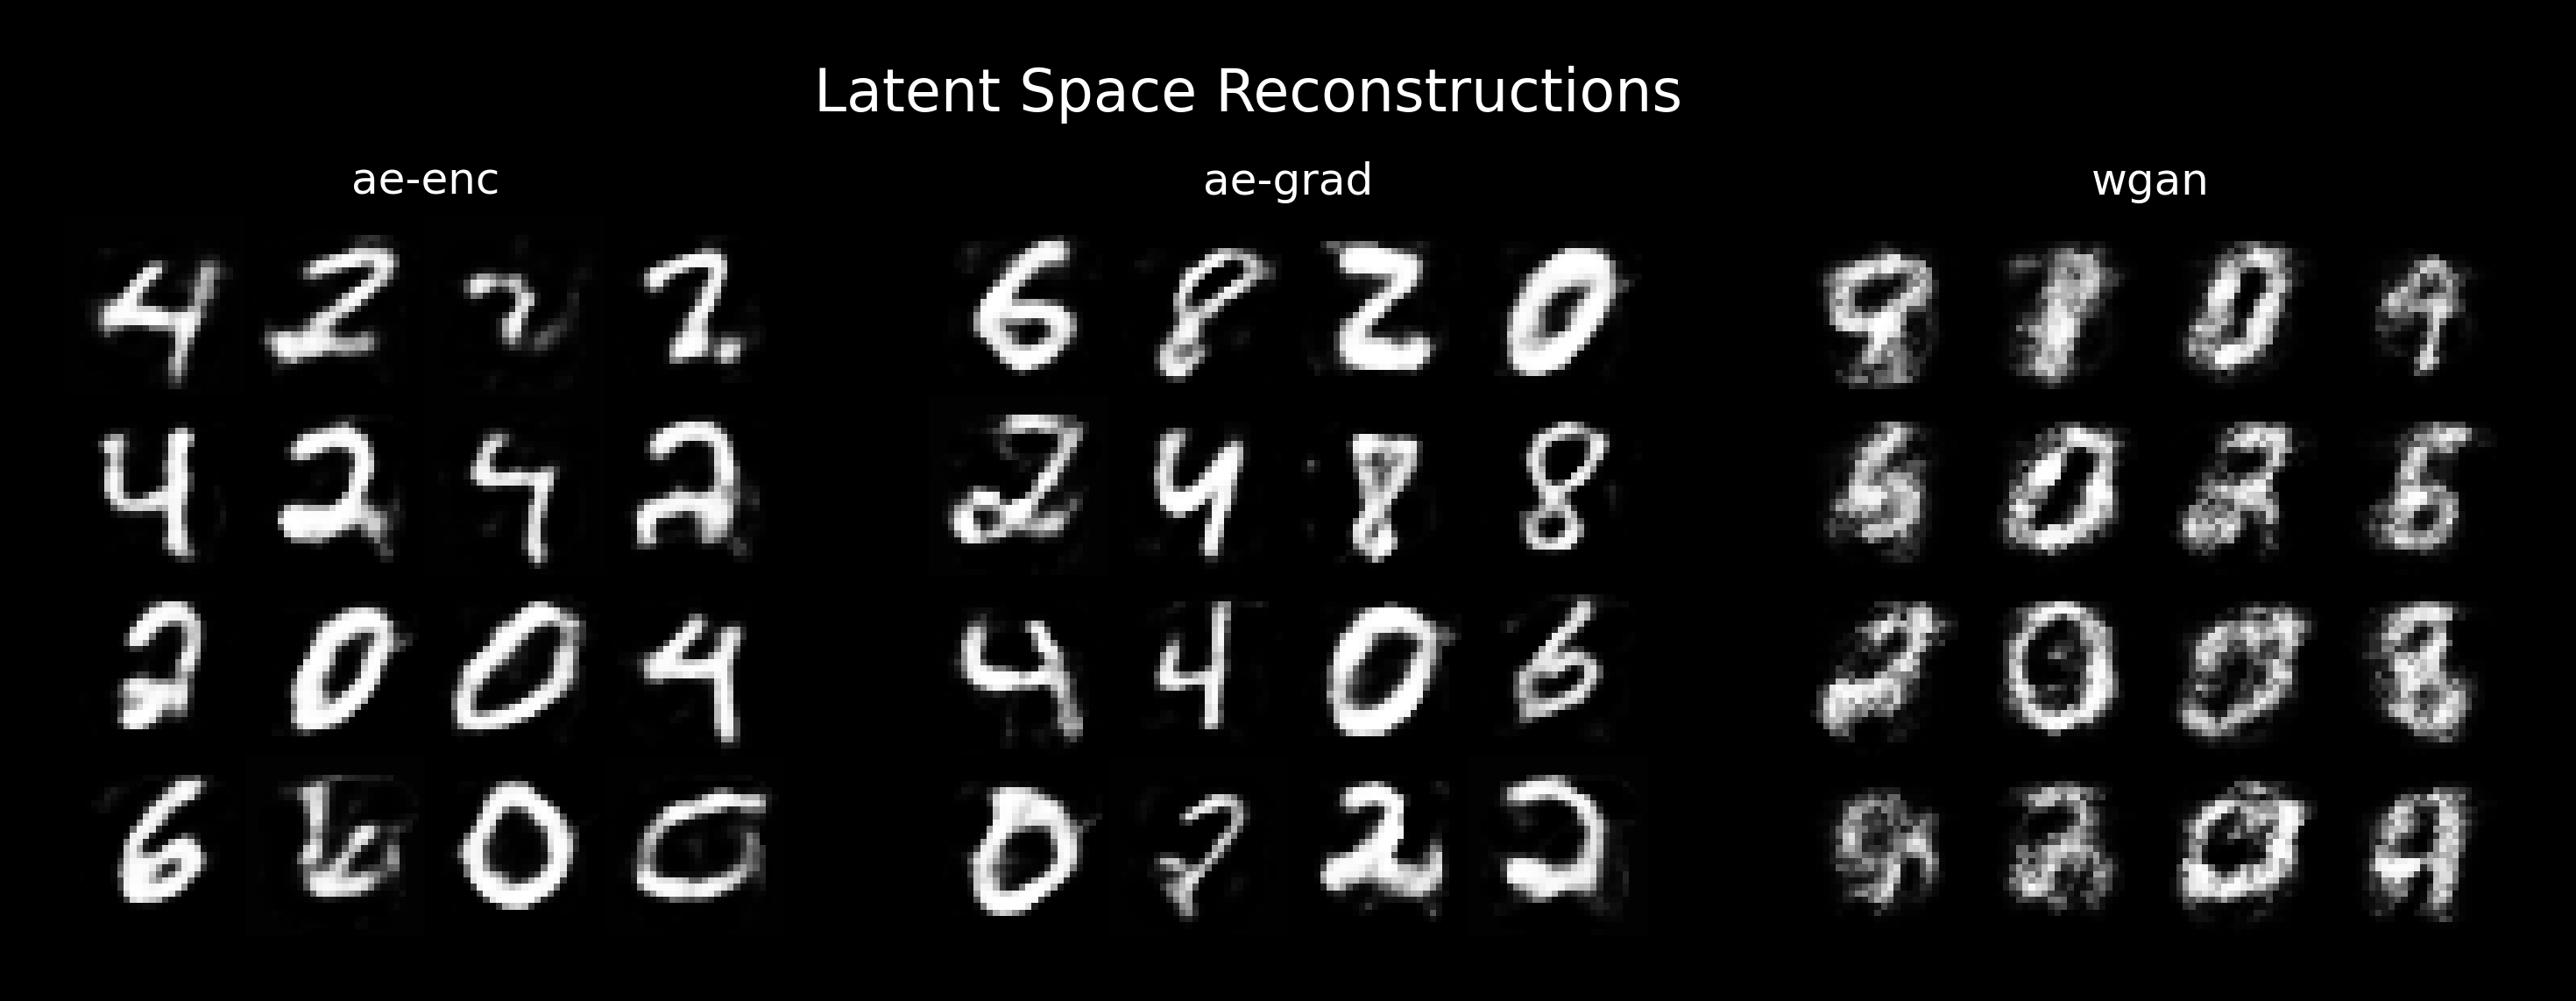
\includegraphics[width=0.8\columnwidth]{images/latent_samples.png}
    \caption{Sample reconstructions from different latent extraction methods.}
    \label{fig:latent_samples}
\end{figure*}



\begin{figure*}[!h]
    \centering
    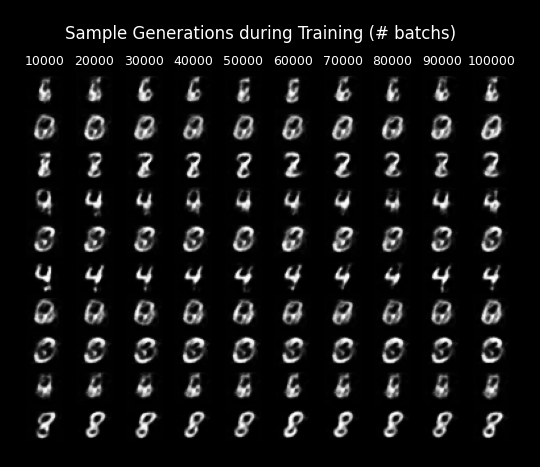
\includegraphics[width=0.6\columnwidth]{images/during_train_inf.png}
    \caption{Generated images during the training of the ae-grad-VAE model. $\epsilon = \infty$.}
    \label{fig:during_train_inf}
\end{figure*}

\subsection{Latent Extraction}
We found that the gradient ascent (ae-grad) algorithm was able to find latent representations which generate high quality reconstructions (Fig. \ref{fig:latent_samples}). We can also see that the projected gradient ascent (wgan-grad) method found latents with reasonable quality, given the poorly hyperparameter tuned public GAN model. This resulted in our later wgan-grad-VAE models failing to produce anything other than a single mode, even without privacy. We believe that with improved public GAN training, the wgan-grad-VAE method would be able to produce results comparable to those of ae-grad-VAE.

We use 200,000 iterations for both algorithms in all experiments (Fig. \ref{fig:gradient_ascent}). Both of these latent extraction methods was only ran once for the private data and took under 30 minutes to complete.

Additionally, we found that the reconstructions from private data encoded using the public autoencoder (ae-enc) were of fairly high quality (Fig. \ref{fig:latent_samples}), and took less than a minute to complete. However, we also found it difficult to train a VaeGM model (ae-enc-VAE) on these encoded latents, and the models were only able to output a single mode. We believe that this may be due to the encoded latents being in an non-well-behaved space (e.g. unsmooth), whereas gradient ascent methods are more likely to find a well-behaved local minimum. 

Since none of our *-GAN methods were successful, this leaves us with only a functional ae-grad-VAE model, which we will now analyze (Fig. \ref{fig:during_train_inf}).

\begin{figure*}[!h]
    \centering
    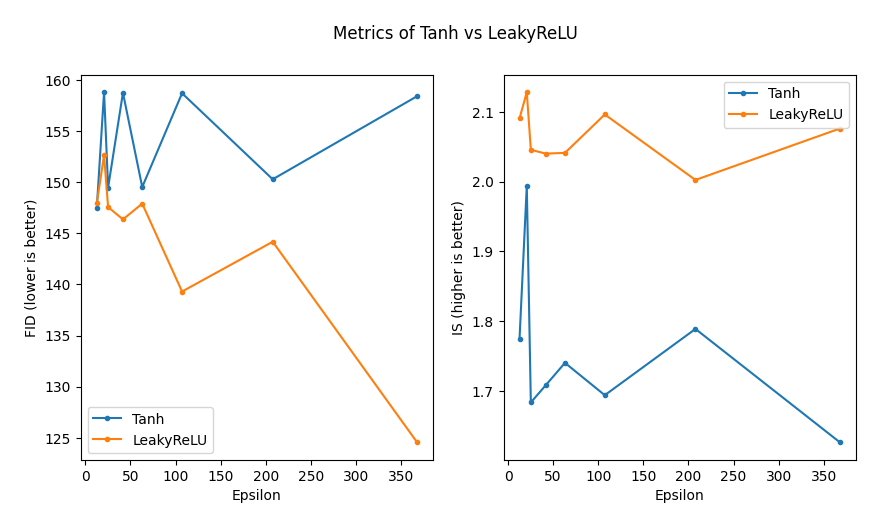
\includegraphics[width=0.8\columnwidth]{images/activation.png}
    \caption{Comparison between tanh and LeakyReLU activation functions.}
    \label{fig:activation}
\end{figure*}


\subsection{Activation Functions}
In our ae-grad-VAE experiments, we compared the performance of tanh and LeakyReLU (Slope of $0.2$) activation functions. Fig. \ref{fig:activation} shows the performance of the best tanh and LeakyReLU models at each $\epsilon$. We found that the LeakyReLU activation function was able to produce better results at higher $\epsilon$ settings, but tanh performed comparably to LeakyRelu at lower ones, with a tanh model slightly beating the best LeakyReLU model at the lowest $\epsilon$ in terms of FID. 

We believe that this is due to the suggested idea from Papernot et al. \cite{sig} that, since the tanh function has bounded range, it is better suited for small gradient norm clipping values, which is usually the case of smaller $\epsilon$ settings. Based on this, we think that if we explored lower $\epsilon$ settings, we would find that tanh would likely perform comparably or even better than LeakyReLU. 

A minor drawback of tanh is the computational cost of computing the gradient of the tanh function, which is more expensive than the gradient of the LeakyReLU function which is only ever 1 or 0.2. We found that tanh generally took about 10-20\% longer to train than LeakyReLU, but this was not a significant factor in our experiments.


\begin{figure*}[!h]
    \centering
    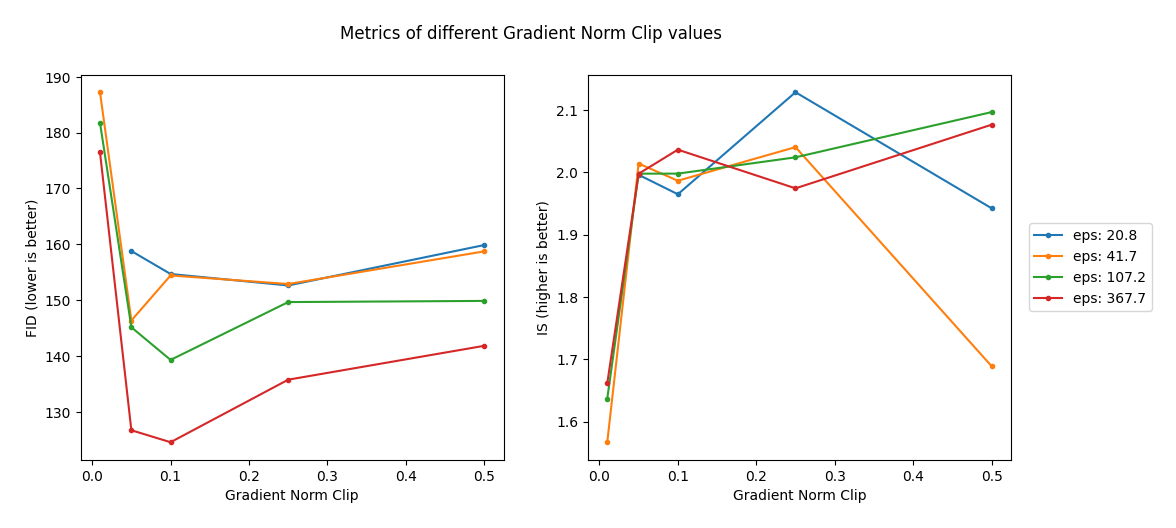
\includegraphics[width=0.9\columnwidth]{images/c_p.png}
    \caption{Comparison between different Gradient Norm Clipping values.}
    \label{fig:clip}
\end{figure*}


\subsection{Gradient Norm Clips at Different $\epsilon$ Settings}
We also analyze the difference in which gradient norm clipping value is best at each epsilon level (See Fig. \ref{fig:clip}). We found that, for our hyperparameter settings, the best gradient norm clipping value was usually between $0.05$ and $0.1$. Note that performance drops sharply at a value of $0.01$, and degrades more slowly as the clip value increases. 

This hyperparameter was very important to tune, as the gradient clip value determines the sensitivity of the entire model, which in turn, affects how much noise we need to add to the gradients. In our tuning, we aimed to decrease this value as much as possible in order to add less noise without sacrificing too much utility in the resulting gradients. 





%%%%%%%%%%%%%%%%%%%%%%%%%%%%%%%%%%%%%%%%%%%%%%%%%
\section{Discussion and Conclusions}
In this project, we explored several variations of the Differential Privacy for Model Inversion (DPMI) framework \cite{dpmi}, utilizing autoencoders and VAEs in place of GANs for generating synthetic data. Our results demonstrated the instability of training GAN-based methods, and explored a more stable approach to generate synthetic data while maintaining privacy, as measured by Inception Score (IS) and Fréchet Inception Distance (FID).

One of the main advantages of using autoencoders and VAEs in the DPMI framework is their simplicity and stability compared to GANs, which are often difficult to train as a result of mode collapse issues and long training times. Another advantage of the VAE in particular is the ability to match the GAN in its ability to generate an infinite amount of synthetic data once trained, which is critical in downstream applications requiring large amounts of data such as data analysis and machine learning. 

As is the case with other DP methods, it is important to consider the trade-offs between privacy and utility. As the level of privacy and added noise increases, the utility of the generated synthetic data will decrease, as we can see in \ref{fig:generated_data}. Therefore, finding the right balance between privacy and utility is an important decision to make in applying our methods in real-world scenarios.

Our results showed that autoencoders and VAEs can potentially be viable alternatives to GANs in the DPMI framework, providing simplicity and stability in generating synthetic data for privacy-preserving applications, especially in applications where there is insufficient data or resources to train the GANs required in vanilla DPMI. 



%%%%%%%%%%%%%%%%%%%%%%%%%%%%%%%%%%%%%%%%%%%%%%%%%
\section{Open Problems and Future Work}
% and what is required to achieve it
The main path of improvement for the proposed DPMI modifications would be through the exploration of more complex models throughout all the experiments, as we largely used simple 1-2 layer fully connected neural networks. Additionally, a deeper and wider hyperparameter search across the different settings will likely result in far better metrics comparable to those in the original DPMI paper. Moreover, it would be beneficial to see an expanded set of metrics such as downstream model accuracy or robustness to model inference attacks \cite{mi_attack} \cite{mi_attack_gan}, which better captures the utility of the method in downstream applications compared to IS and FID.

In the context of the DPMI framework and DP generative models in general, scalability and efficiency of privacy-preserving methods in real-world deployments are significant open problems. One popular method of achieving this is through Collaborative Deep Learning \cite{collab}, a process which allows multiple parties to jointly learn a model without sharing their individual datasets. However, there have been proposed attacks which prove to be effective against these collaborative deep learning methods \cite{collab_attack}. Further research is needed to develop distributed, federated, or decentralized methods capable of training robust generative models in a scalable manner, especially on large datasets. Classical cryptographic methods like multiparty computation or fully homomorphic encryption could potentially be used as solutions, but they are computationally costly and still have vulnerabilities \cite{collab_attack}. Therefore, exploring different granularities of differential privacy, such as at the user or device level, could be a potential solution for privacy-preserving collaborative learning. 

Another open problem is the interpretability and explainability of DP generative models. While these models can generate synthetic data with privacy guarantees, comprehending the relationship between the generated data and the original data, as well as the underlying data distribution, can be challenging. Developing techniques for interpreting and explaining the outputs of these models while still preserving the privacy of private data could greatly enhance the trust and usability of these methods in sensitive real-world applications where concerns about biases are prominent. Addressing this challenge could contribute to the responsible and ethical use of differential privacy generative models in practical settings.

Lastly, as the adoption of differential privacy grows in popularity as a means of providing provable privacy guarantees, there is an increasing need for practical guidelines and best practices for real-world deployments of DP generative models. While these models are valuable for privacy-preserving data generation, their practical implementation and hyperparameter settings can be complex and challenging to comprehend. Establishing guidelines for model selection, hyperparameter tuning, and privacy budget allocation can assist practitioners in effectively deploying these models with a clear understanding of the privacy guarantees they offer, avoiding a false sense of security.






\newpage
\bibliography{ref}
\bibliographystyle{abbrv}


\section{Appendix}

% Table of hyperparameters
\begin{table}[!h]
    \centering
    \begin{tabular}[!h]{|c|c|}
        \hline
        \textbf{Hyperparameter} & \textbf{Values}\\
        \hline
        \hline
        \multicolumn{2}{|c|}{\textbf{Fixed for all experiments}}\\
        \hline
        Batch Size & 64, 32\\
        Activation & Tanh, LeakyReLU(0.2)\\
        Public Latent Size & 100\\
        Optimizer & Adam(0.5, 0.9, weight decay 1e-6)\\
        \hline
        \hline
        \multicolumn{2}{|c|}{\textbf{Public GAN}}\\
        \hline
        Model Architecture & [[256], [128], [128, 128]] FC hidden layers, 3 Layer CNN (32, 4, 2, 1)\\
        Learning Rate & 5e-05, 5e-04\\
        Discriminator Update Ratio & 5:1, 3:1\\
        Generator Updates & 5e5\\
        GAN Variants & WGAN, WGAN-GP\\
        \hline
        \hline
        % 
        % 
        \multicolumn{2}{|c|}{\textbf{Public Autoencoder}}\\
        \hline
        Model Architecture & [128] FC hidden layers\\
        Learning Rate & 5e-04\\
        Epochs & 1000\\
        \hline
        \hline
        % 
        % 
        \multicolumn{2}{|c|}{\textbf{Private DP-GAN (WGAN)}}\\
        \hline
        Model Architecture & [[128], [96], [32], [16], [16, 12], [12, 4, 4]] FC layers\\
        Learning Rate & 5e-06, 1e-05, 5e-05\\
        Noise Multiplier & 0.0, 0.05, 0.1, 0.2\\
        Clipping Norm & 0.005, 0.01\\
        Discriminator Update Ratio & 5:1, 3:1\\
        Private Latent Size & 32, 64\\
        \hline
        \hline
        % 
        % 
        \multicolumn{2}{|c|}{\textbf{Private VaeGM}}\\
        \hline
        Model Architecture & [64] FC hidden layers\\
        Learning Rate & 0.005, 0.01, 0.02\\
        Noise Multiplier & 0.0, 0.01, 0.05, 0.1, 0.2, 0.3, 0.4, 0.5, 0.6\\
        Clipping Norm & 0.001, 0.005, 0.01, 0.05, 0.1, 0.25, 0.5\\
        Batch Updates & 1000, 10000, 48000, 100000\\
        Private Latent Size & 32\\
        \hline
        % \hline
        % 
        % 
        % \multicolumn{2}{|c|}{Public DP-GAN}\\
        % \hline
        % \hline
        % 
        % 
    \end{tabular}
    \caption{Hyperparameters used in the experiments.}
    \label{table:hyperparameters}
\end{table}

\begin{figure*}[!h]
    \centering
    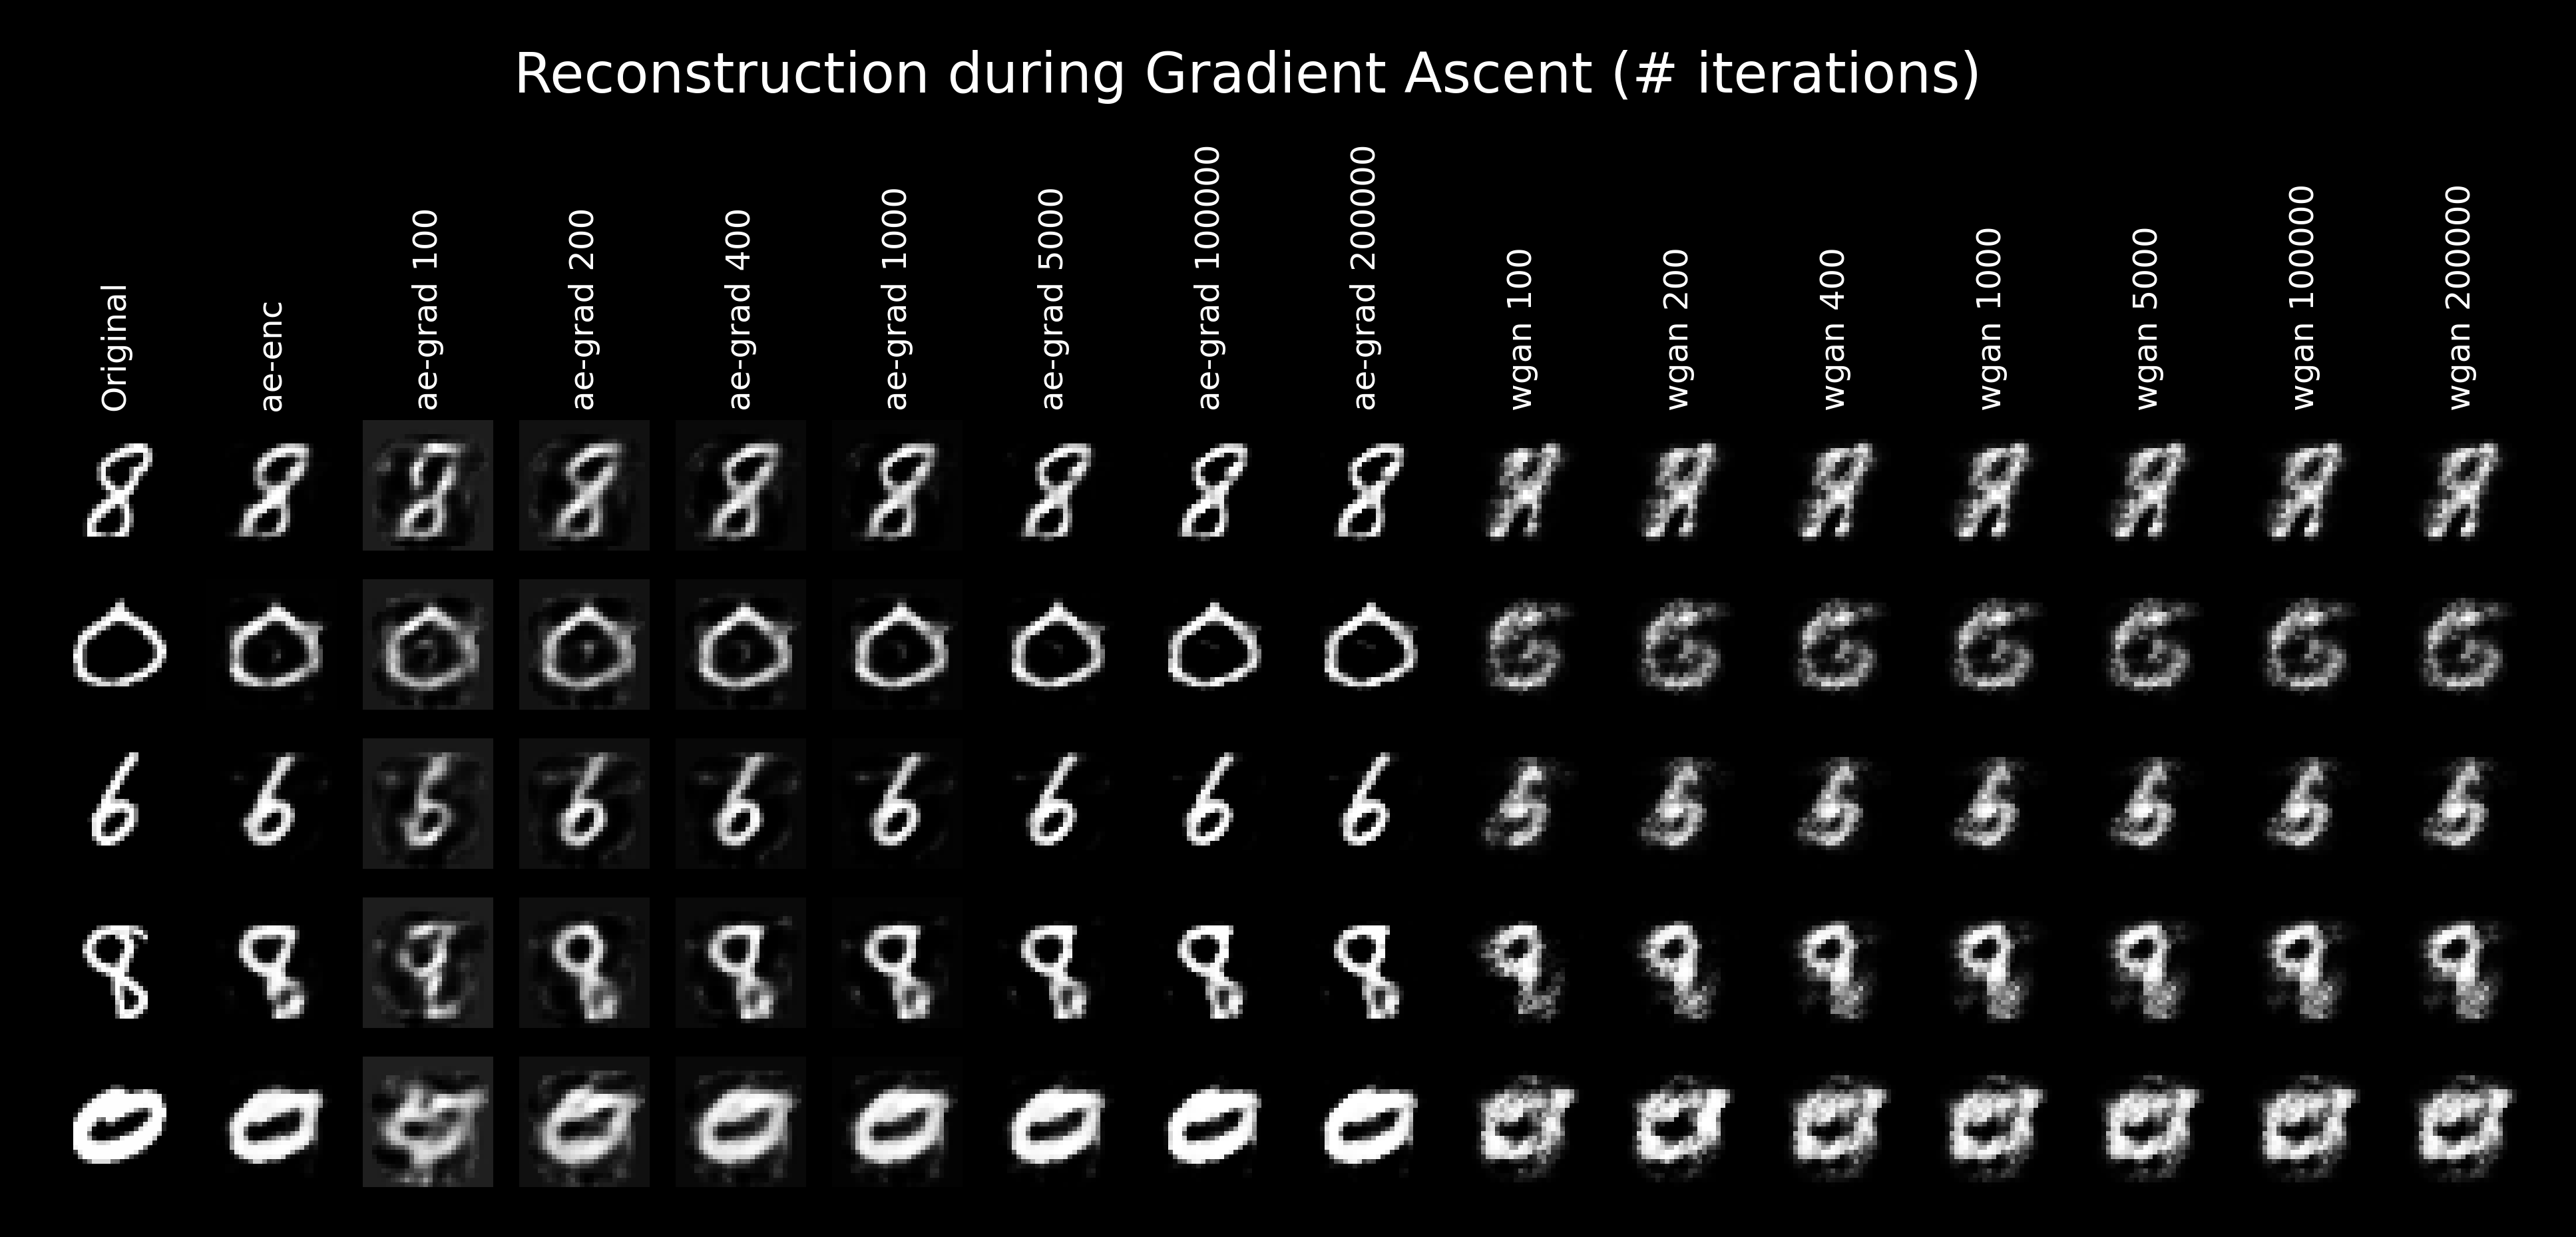
\includegraphics[width=0.8\columnwidth]{images/gradient_ascent.png}
    \caption{Reconstructions at different iteration steps of the gradient ascent algorithm.}
    \label{fig:gradient_ascent}
\end{figure*}



\begin{figure*}[!h]
    \centering
    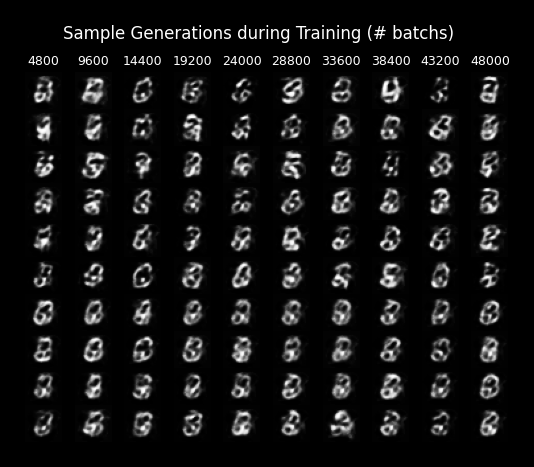
\includegraphics[width=0.6\columnwidth]{images/during_train_367_7.png}
    \caption{Generated images during the training of the ae-grad-VAE model. $\epsilon = 367.7$.}
    \label{fig:during_train_367_7}
\end{figure*}




\begin{figure*}[!h]
    \centering
    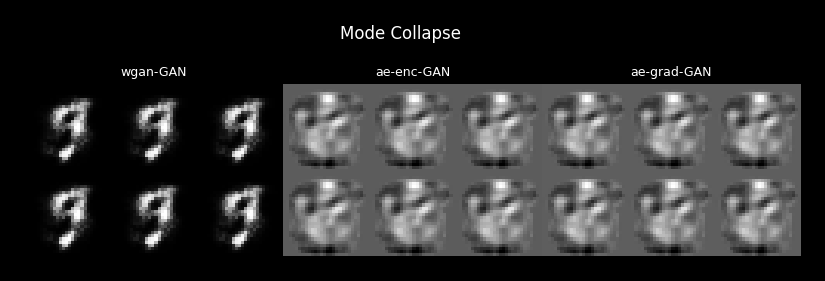
\includegraphics[width=\columnwidth]{images/mode_collapse.png}
    \caption{Reconstructions from mode collapsed models.}
    \label{fig:mode_collapse}
\end{figure*}   









\end{document}